% RLHF Schematic — simplified reproduction of Christiano et al. (2017) Figure 1
% Shows: RL Algorithm <-> Environment loop, Reward Predictor with human feedback

\documentclass{article}
\usepackage[margin=0.3cm, paperwidth=16cm, paperheight=9cm]{geometry}
\usepackage{tikz}
\usetikzlibrary{positioning, arrows.meta, calc}
\pagestyle{empty}

\begin{document}

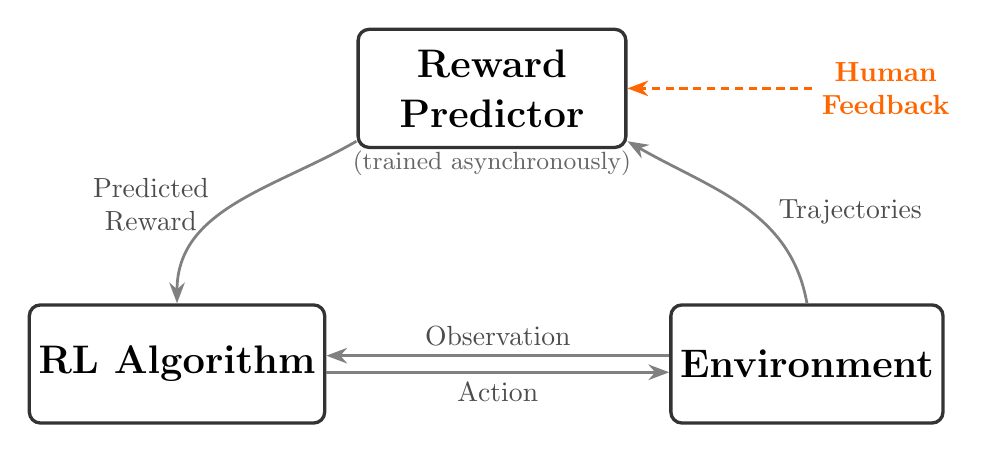
\begin{tikzpicture}[
    box/.style={
        rectangle,
        draw=black!80,
        fill=white,
        minimum width=3.4cm,
        minimum height=1.5cm,
        font=\Large\bfseries,
        rounded corners=4pt,
        align=center,
        line width=1.2pt
    },
    arrow/.style={
        ->,
        >=Stealth,
        line width=1.0pt,
        color=black!50
    },
    dasharrow/.style={
        ->,
        >=Stealth,
        line width=1.0pt,
        densely dashed,
        color=orange!80!red
    },
    lbl/.style={
        font=\normalsize,
        color=black!70,
        align=center
    },
    humanlbl/.style={
        font=\normalsize\bfseries,
        color=orange!80!red,
        align=center
    }
]

% Nodes
\node[box] (rl)  at (0,   0)   {RL Algorithm};
\node[box] (env) at (8, 0)   {Environment};
\node[box] (rp)  at (4, 3.5) {Reward\\Predictor};
\node[font=\small, color=black!60] at (4, 2.55) {(trained asynchronously)};

% RL <-> Environment arrows (action right, observation left — matching Christiano et al.)
\draw[arrow] ([yshift=-3pt] rl.east)  -- node[lbl, below] {Action}
             ([yshift=-3pt] env.west);
\draw[arrow] ([yshift= 3pt] env.west) -- node[lbl, above] {Observation}
             ([yshift= 3pt] rl.east);

% Environment -> Reward Predictor (trajectories)
\draw[arrow] (env.north) to[out=100, in=-30]
    node[lbl, right, pos=0.45, xshift=6pt] {Trajectories} ($(rp.south east) + (0, 0.1)$);

% Reward Predictor -> RL Algorithm (predicted reward)
\draw[arrow] ($(rp.south west) + (0, 0.1)$) to[out=210, in=90]
    node[lbl, left, pos=0.5, xshift=-6pt] {Predicted\\Reward} (rl.north);

% Human feedback (dashed, from right)
\node[humanlbl] (human) at (9, 3.5) {Human\\Feedback};
\draw[dasharrow] (human.west) -- (rp.east);

\end{tikzpicture}

\end{document}
